\label{chapter-5}
In the previous chapter, a set of suggestions for improving a BPMN diagram was listed. As was also mentioned, not all of these improvements can be automated. 

This chapter will provide an example of how the mentioned not automatable and automatable suggestions can be applied together to an existing BPMN model. 

At first, the example BPMN model used for this case study and the evaluation that is done by the software on this BPMN will be explained. Finally, all suggestions as they are listed in section \ref{last} will be implemented one by one, using the software evaluation as an aid. 

\section{The Example Model}
The used BPMN model for this chapter will be a fictitious client registration process that was adapted from a real live process used in the telecommunication sector to be used in this thesis. The graphical representation of the process model can be found in figure \ref{fig:example-process}. The full \textit{.bpmn} file of this process can be accessed in the GitHub repository\cite{appendix-registration-1}. 

\begin{figure}[H]
	\centering
	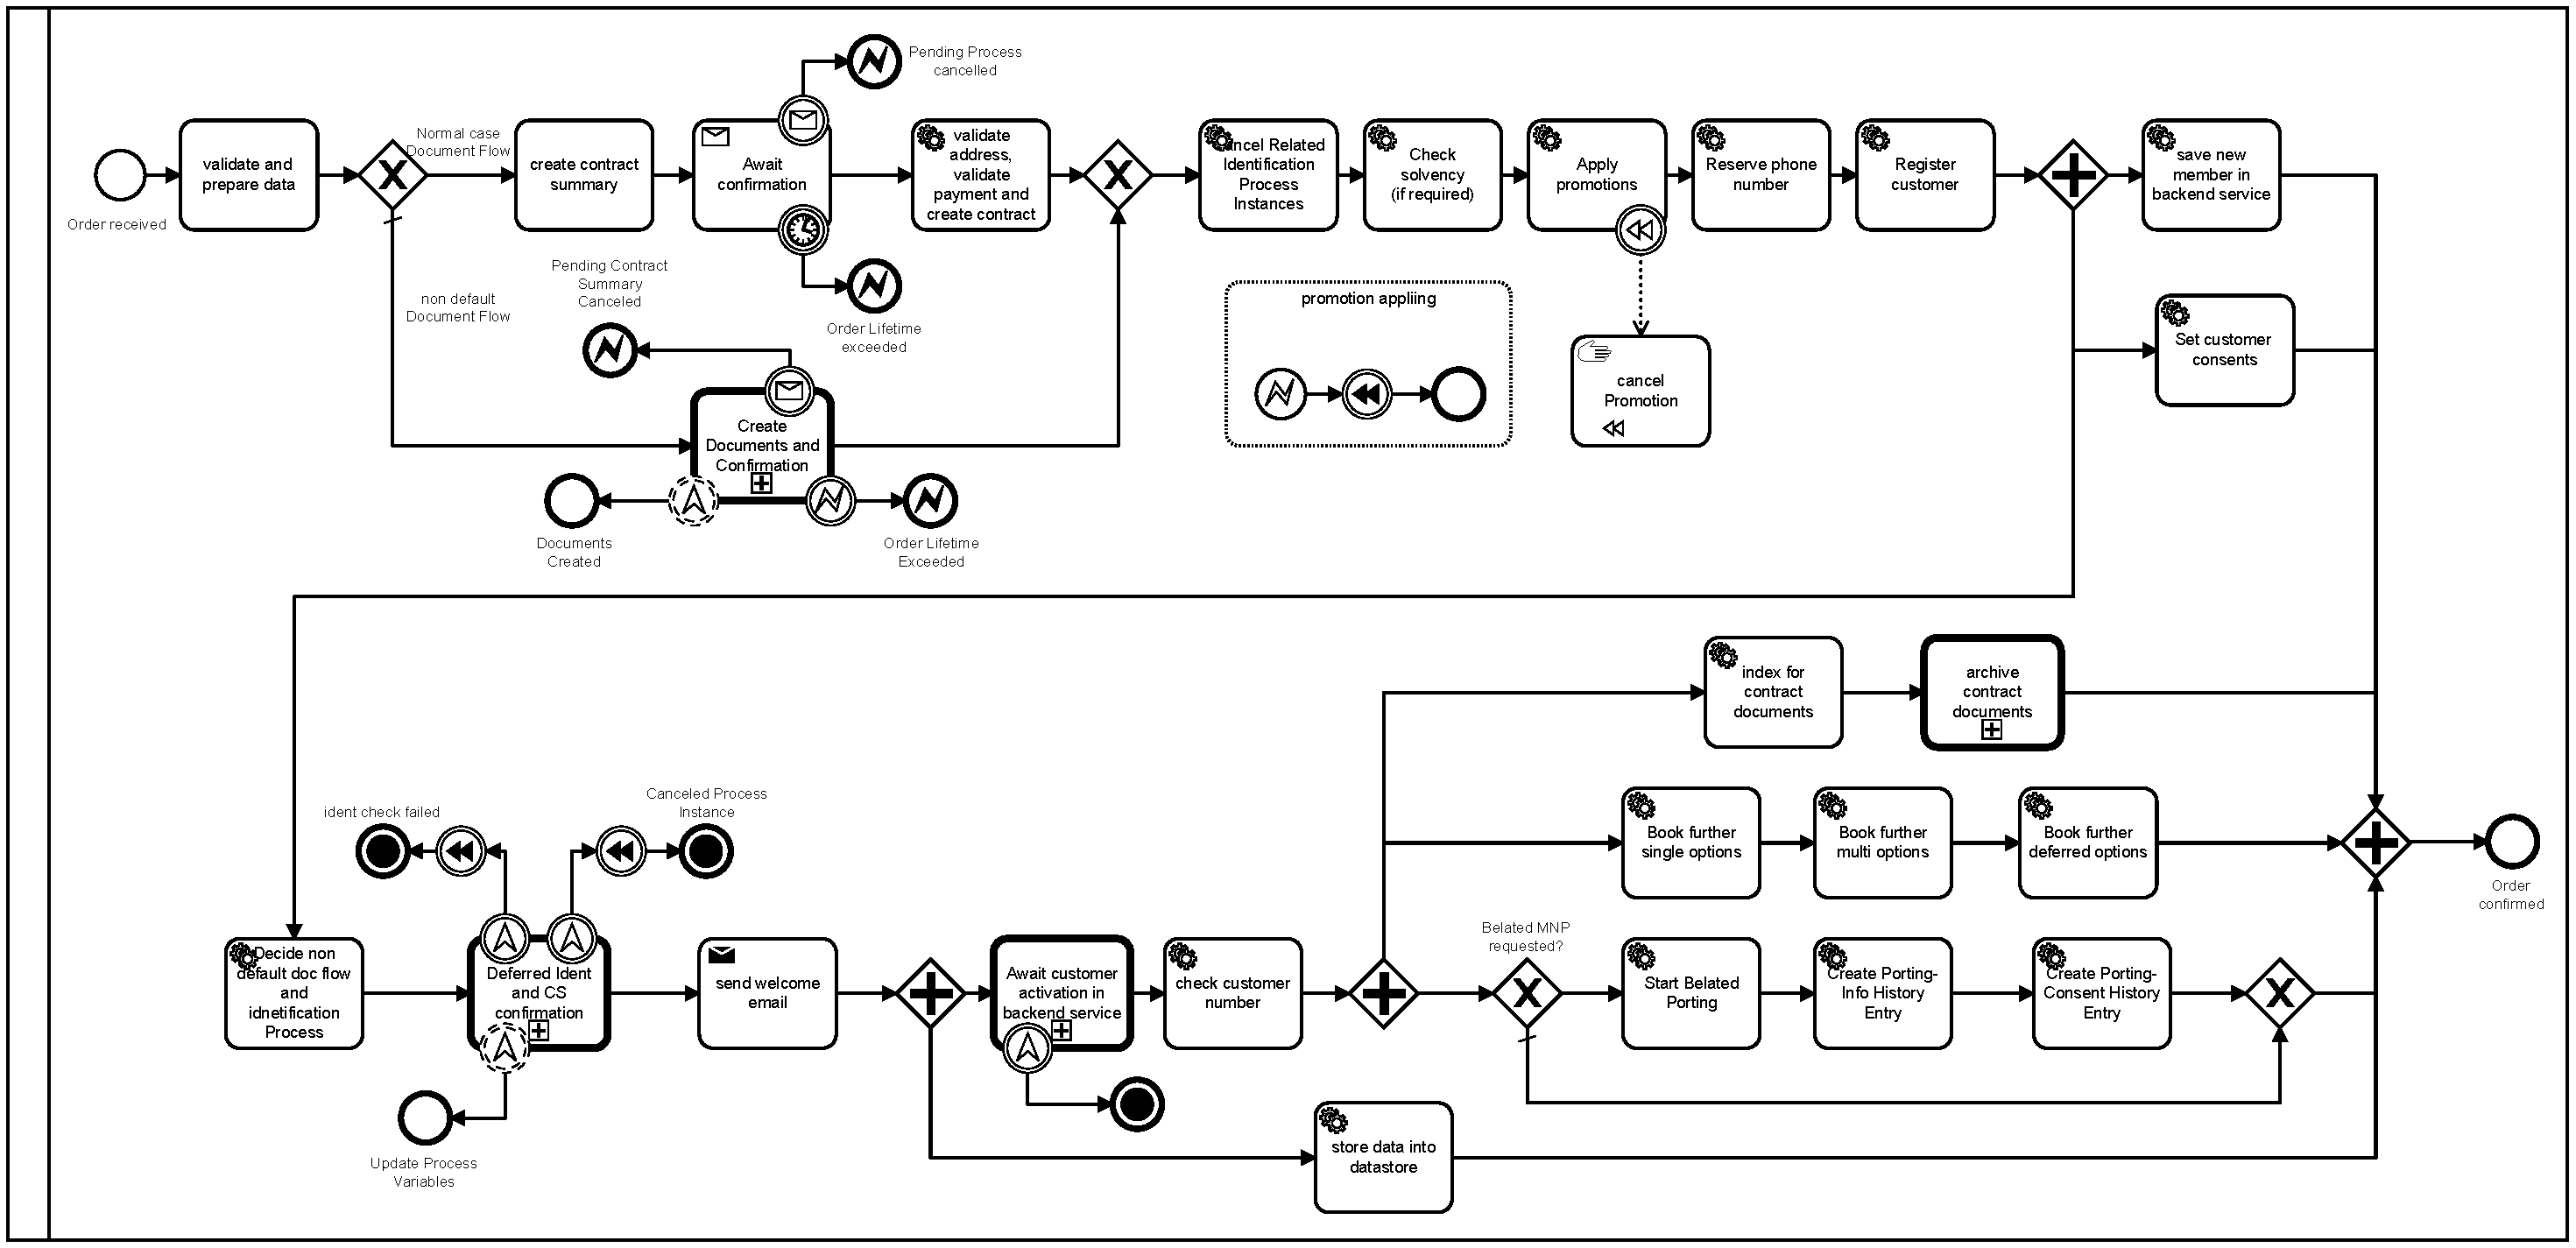
\includegraphics[width=1.7\columnwidth, angle=90]{graphics/register-customer/1-registercustomer-bpmn.pdf}
	\caption{Adapted customer registrations process} 
	\label{fig:example-process} 
\end{figure}

\section{Evaluation by the Software}
To evaluate the best practices that were implemented the BPMN Model was given as input for the software. The following output for each suggestion/rule was given. The full output can be found in the appendix section \ref{app-output}.
\paragraph{Comply with Naming Conventions}~\\
As described in chapter \ref{naming-con}, this algorithm scans the BPMN model for events, tasks, or gateways that have more than five words in their label. The following list of elements is returned that violate this rule:
\begin{lstlisting}[language=json,label=lst:naming]
	"affectedElements": [
	{
		"id": "ServiceTask_DefaultDocWorkflowPostAwaitConfirmation",
		"name": "validate address, validate payment and create contract",
		"type": "Task"
	},
	{
		"id": "DecideIdAndCsProcess",
		"name": "Decide non default doc flow and idnetification Process",
		"type": "Task"
	},
	{
		"id": "save_member_for_riskident",
		"name": "save new member in backend service",
		"type": "Task"
	}
\end{lstlisting}


\paragraph{Eliminate Manual Tasks}~\\
When searching for manual tasks in the process (see section \ref{soft-manual}), only one can be identified and is returned:
\begin{lstlisting}[language=json,label=lst:manual]
	"affectedElements": [
	{
		"id": "data_to_warehouse",
		"name": "store data into datastore",
		"type": "Task"
	}
\end{lstlisting}
\paragraph{Merge Consecutive Tasks Handled by the Same Resource}~\\
Another rule that was implemented was that no two consecutive tasks should be processed by the same resource. The software identified the following tasks that could be merged with its successor:
\begin{lstlisting}[language=json,label=lst:merge]
	"affectedElements": [
	{
		"id": "CancelRelatedWebIdent",
		"name": "Cancel Related Identification Process Instances",
		"type": "Task"
	},
	{
		"id": "ReserveMsisdn",
		"name": "Reserve phone number",
		"type": "Task"
	},
	{
		"id": "BookAutoTopups",
		"name": "Book further multi options",
		"type": "Task"
	},
	{
		"id": "ServiceTask_0p0tajd",
		"name": "Start Belated Porting",
		"type": "Task"
	},
	{
		"id": "ServiceTask_0e2r82f",
		"name": "Create Porting-Info History Entry",
		"type": "Task"
	},
	{
		"id": "BookSingleTopups",
		"name": "Book further single options",
		"type": "Task"
	}
	]
\end{lstlisting}
\paragraph{Replace Combinations of Parallel and Exclusive Gateways With Inclusive Gateways}~\\
As described in section \ref{inc-sw} it is preferred to use inclusive gateways instead of combining parallel and exclusive gateways. The only element that violates that rule in the given BPMN is returned:
\begin{lstlisting}[language=json]
	"affectedElements": [
	{
		"id": "ParallelGateway_0crudor",
		"name": null,
		"type": "Gateway"
	}
	]
\end{lstlisting}
\section{Apply Suggestions for Improvement}\label{improvements}
The following section will give an introduction on how the suggestions mentioned in section \ref{last} can be applied to the process in figure \ref{fig:example-process}. 
\subsection{Comply with Naming Conventions}
Based on the naming conventions defined in section \ref{naming}, unnamed tasks, events, and gateways were named and elements returned in listing \ref{lst:naming} were renamed. In figure \ref{fig:naming-org} a segment of the example BPMN, where the naming conventions are violated, is shown, and figure \ref{fig:naming-new} shows the corresponding changes after renaming. 

\begin{figure}[H]
	\centering
	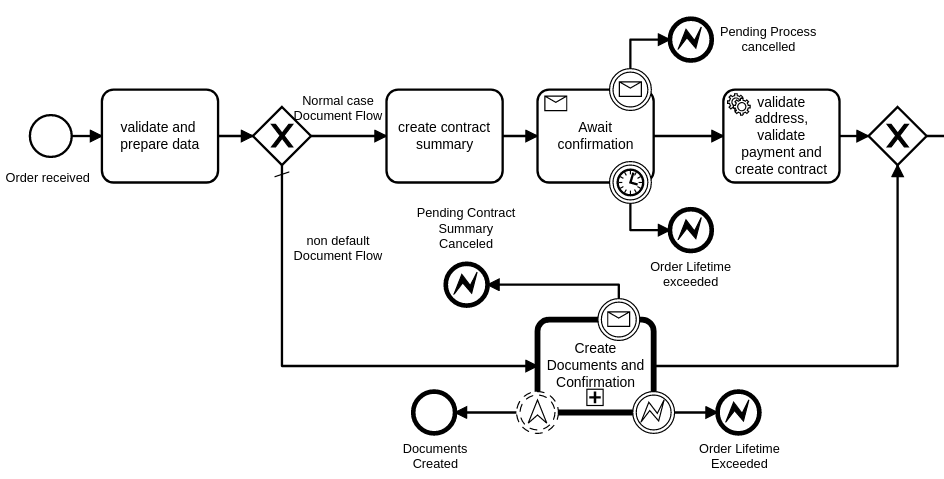
\includegraphics[width=0.9\columnwidth]{graphics/case-study-naming-org}
	\caption{Segment of the BPMN model in figure \ref{fig:example-process}}
	\label{fig:naming-org}
\end{figure}

\begin{figure}[H]
	\centering
	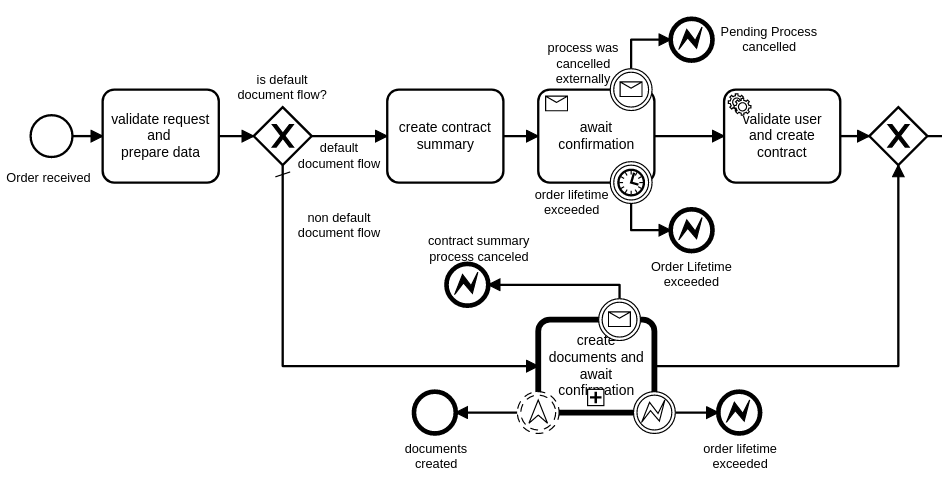
\includegraphics[width=0.9\columnwidth]{graphics/case-study-naming-new}
	\caption{Segment \ref{fig:naming-org} with changed element labels in order to satisfy naming conventions}
	\label{fig:naming-new}
\end{figure}

The full renaming change can be found in the appendix chapter \ref{BPMN-improvements} in figure \ref{fig:process-renaming}. The full XML representation of this process can be found in the GitHub repository\cite{appendix-registration-2}.

\subsection{Eliminate Manual Tasks}
The only manual task in this BPMN model is the \textit{cancel promotion} task. Canceling promotions can only be done manually by a service agent in this fictitious case and can therefore not be automated. In this case, the manual task can be changed into a \textit{user task} and the advantages of a worklist handler can be utilized as described in section \ref{manual}.
The original segment with the manual task can be seen in figure \ref{fig:manual-org}. The corresponding change in this section is shown in figure \ref{fig:manual-new}. 


\begin{minipage}[t]{0.5\textwidth}
	\begin{figure}[H]
		\centering
		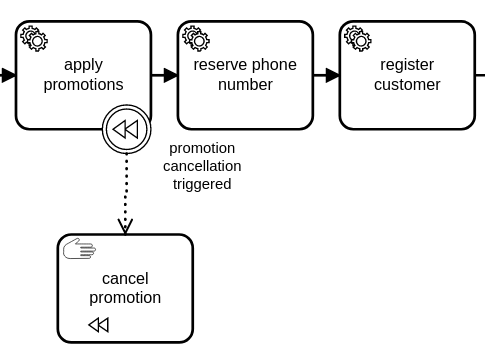
\includegraphics[width=0.8\textwidth]{graphics/case-study-manual-org}
		\caption{Segment of the BPMN model in figure \ref{fig:example-process} with the manual task}
		\label{fig:manual-org}
	\end{figure}
\end{minipage}
\begin{minipage}[t]{0.5\textwidth}
	\begin{figure}[H]
		\centering
		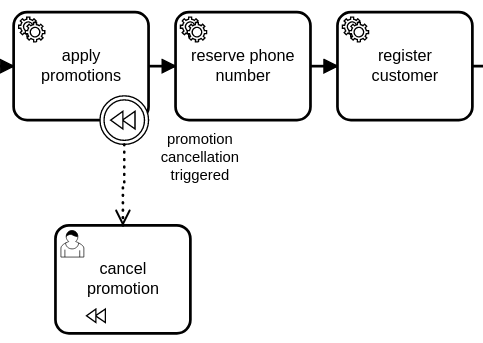
\includegraphics[width=0.8\textwidth]{graphics/case-study-manual-new}
		\caption{Segment that is shown in figure \ref{fig:naming-org} with changing the manual tasks to a user task}
		\label{fig:manual-new}
	\end{figure}
\end{minipage}

The fully changed BPMN file can be found in the appendix chapter \ref{BPMN-improvements} in figure \ref{fig:process-manual}. The full XML representation of this process can be found in the GitHub repository\cite{appendix-registration-3}.
\subsection{Complete the Process Model}
This fictional model covers all cases and error scenarios that can happen in this process.

\subsection{Extend Automation Boundaries}
Since the process model is, apart from the \textit{cancel promotion} task, already fully automated and this activity is not automatable yet the automation boundaries cannot be extended further. 

\subsection{Merge Consecutive Tasks Handled by the Same Resource}
According to the rules described in section \ref{merge-section}, the list of elements given in \ref{lst:merge} can be merged with their direct successor. The segements of the BPMN model with the listed elements can be found in figures \ref{fig:merge-1-org} and \ref{fig:merge-2-org} and the respective change is shown in figures \ref{fig:merge-1-new} and \ref{fig:merge-2-new}. 
\begin{figure}[H]
	\centering
	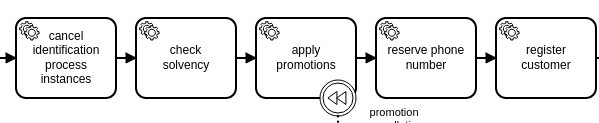
\includegraphics[width=0.8\textwidth]{graphics/case-study-merge-org-1}
	\caption{Segment of the BPMN model \ref{fig:example-process} with consecutive service tasks}
	\label{fig:merge-1-org}
\end{figure}

\begin{figure}[H]
	\centering
	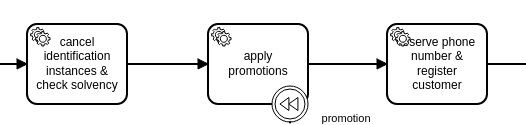
\includegraphics[width=0.8\textwidth]{graphics/case-study-merge-new-1}
	\caption{Segment that is shown in figure \ref{fig:merge-1-org} with merged consecutive service tasks}
	\label{fig:merge-1-new}
\end{figure}

\begin{minipage}[t]{0.5\textwidth}
	\begin{figure}[H]
		\centering
		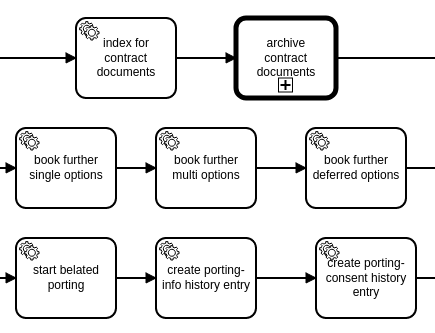
\includegraphics[width=0.95\textwidth]{graphics/case-study-merge-org-2}
		\caption{Segment of the BPMN model \ref{fig:example-process} with consecutive service tasks}
		\label{fig:merge-2-org}
	\end{figure}
\end{minipage}
\begin{minipage}[t]{0.5\textwidth}
	\begin{figure}[H]
		\centering
		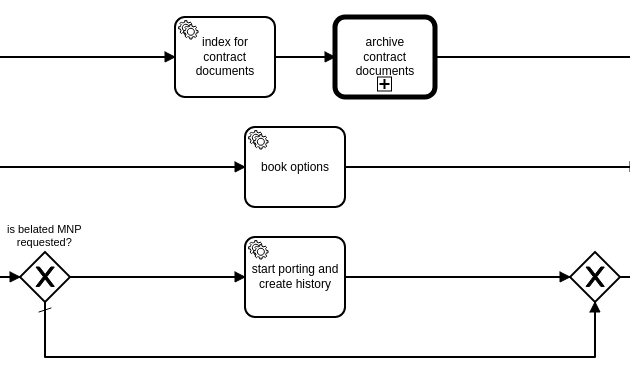
\includegraphics[width=0.95\textwidth]{graphics/case-study-merge-new-2}
		\caption{Segment that is shown in figure \ref{fig:merge-2-org} with merged consecutive service tasks}
		\label{fig:merge-2-new}
	\end{figure}
\end{minipage}

The changes in the BPMN file can be found in the appendix chapter \ref{BPMN-improvements} in figure \ref{fig:process-merge}. The full XML representation of this process can be found in the GitHub repository\cite{appendix-registration-4}.

\subsection{Replace Combinations of Parallel and Exclusive Gateways With Inclusive Gateways}
The only case in this BPMN model where a combination of parallel and exclusive gateways was used instead of an inclusive gateway is in the segment shown in figure \ref{fig:exclusive-org}. The corresponding change in this section of the model is shown in figure \ref{fig:exclusive-new}. 


\begin{figure}[H]
	\centering
	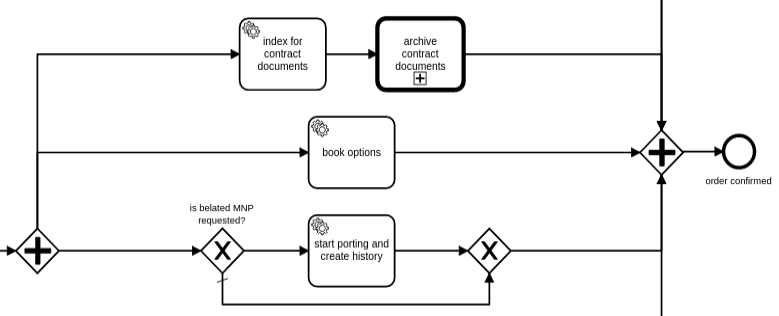
\includegraphics[width=0.8\textwidth]{graphics/case-study-exclusive-org}
	\caption{Segment of the BPMN model in figure \ref{fig:example-process} where parallel and exclusive tasks are combined instead of using an inclusive gateway}
	\label{fig:exclusive-org}
\end{figure}
\begin{figure}[H]
	\centering
	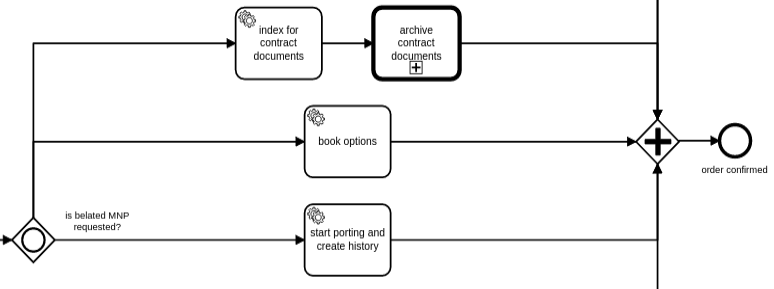
\includegraphics[width=0.8\textwidth]{graphics/case-study-exclusive-new}
	\caption{Segment that is shown in figure \ref{fig:exclusive-org} with using an inclusive gateway}
	\label{fig:exclusive-new}
\end{figure}

The changes in the BPMN file can be found in the appendix chapter \ref{BPMN-improvements} in figure \ref{fig:process-inclusive}. The full XML representation of this process can be found in the GitHub repository\cite{appendix-registration-5}.
\subsection{Perform Value Added Analysis and Waste Elimination}\label{improv-vaa}
To eliminate tasks in a process that have limited value for the customer, a value added analysis as explained in section \ref{vaa} will be performed on the customer registration process. For the value added analysis the last version of the process model will be used after implementing the suggestions discussed now. 

Following the same approach as in seciton \ref{vaa}, the process tasks where categorized in \textcolor{green}{RVA (real value adding)}, \textcolor{orange}{BVA (business value adding)} and \textcolor{red}{NVA (non value adding)}. The colored process is shown in the appendix section \ref{BPMN-vaa} in figure \ref{fig:process-vaa}.

For better understanding, the following list will describe the BVA and NVA activities and why they were categorized as NVA/BVA:

\paragraph{Cancel Identification  Instances \& Check Solvency (BVA)}~\\ 
This activity cancels, in case that a customer registers for the second time, all identification processes of the same customer. Furthermore, the solvency of the customer is checked. Since neither the solvency check, nor the cancellation of identification processes adds value to the customer, but are measures for fraud protection, this activity is marked as business value adding. 
\paragraph{Cancel Promotion (NVA)}~\\ 
The canceling promotions activity has only effect when the registration process fails and promotions have already been booked by the customer. In the case that the promotion stays booked and the customer registration fails, the user cannot use the promotion anyway, therefore this activity was categorized as nonvalue adding.
\paragraph{Determine Appropriate Identification Process (BVA)}~\\ 
There are different ways a customer can be identified. This activity decides based on rules which method is used. Since the whole identification process adds no value to the customer but is used for fraud protection, this activity is marked as business value adding. 
\paragraph{Deferred Ident and Contract Confirmation (BVA)}~\\ 
Depending on the decision taken in the previous activity, this activity performs the identification. 
\paragraph{Create Index for Contract Documents \& Archive Contract Documents (BVA)}~\\ 
Contract documents are not archived for the customer, therefore these two activities are marked as business value adding.

\paragraph{Waste Elimination}~\\
Now that the value of each activity was determined, NVA and BVA tasks can be considered for waste elimination.

As mentioned above, the \textit{cancel promotion} task has neither the real customer nor business value and can therefore be eliminated together with the compensation events that were meant to trigger this activity. 

Another possible waste elimination could be achieved by evaluating the effect of the implemented fraud protection in the following activities and evaluate if simpler measures for fraud protection can be used to achieve similar results.
\begin{itemize}
	\item \textit{Cancel identification  instances \& check solvency (BVA)}, 
	\item \textit{{Determine appropriate identification process (BVA)}} 
	\item \textit{Deferred ident and contract confirmation (BVA)}
\end{itemize}

After eliminating the \textit{cancel promotion} activity and everything related to triggering the compensation, the final process model can be found in figure \ref{fig:process-vaa-waste}.